%RLC_Circuits_P1
Hopefully by now you have learned in your PH 220 class that magnetism is
related to current. Oersted discovered this by accident (so all those
accidents we have experienced in our lab could be telling us something!). If
you don't know yet, you will soon learn that changing magnetic fields can
cause currents. This is called induction. Electronic circuits often use the
ability of currents to cause magnetic fields and the ability of changing
magnetic fields to cause currents. Devices that use magnetic fields are
called \emph{inductors}. I\ will give some review material here on how
magnetic fields, currents, and inductances are related. Lenz's law is
involved, and I\ will assume you know this rule.

We're not going to use our Arduino's today. Instead, we are going to use a
device that measures voltage as a function of time and plots it. We studied
this device briefly back in our second lab. It is called an oscilloscope. We
will get some experience with this device today, and then try to build such
a device with our Arduino in our next lab.

\section{The Model: Self Inductance}

When we put capacitors and resisters in a circuit, we found that the current
did not jump to it's maximum value all at once. There was a time dependence.
But really, even if we just have a resister (and we always have some
resistance!) the current does not reach it's full value instantaneously.
Think of our circuits, they are current loops. So as the current starts to
flow, Lenz's law tells us that there will be an induced emf that will oppose
the flow. The potential drop across the resister in a simple
battery-resister circuit is the potential drop due to the battery emf, \emph{%
minus the induced emf}.

We can use this fact to control current in circuits. To see how, we can
study a new case\begin{figure}[h!]
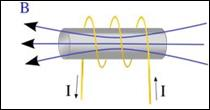
\includegraphics[width=1.977in,height=1.0378in]{PH4CAX4B}
\end{figure}Let's take a coil of wire wound
around an iron cylindrical core. In the picture, we start with a current as
shown in the figure above. If you have studied inductance, you can find the
direction of the $B$-field using our right hand rule number 2. But we now
will allow the current to change. As it gets larger, we know 
\begin{equation*}
\mathcal{E}=-N\frac{d\Phi _{B}}{dt}
\end{equation*}

and we know that as the current changes, the magnitude of the $B$-field will
change, so the flux through the coil will change. So we will have an induced
emf. The induced emf is proportional to the rate of \emph{change} of the
current.%
\begin{equation*}
\mathcal{E}\equiv -L\frac{\Delta I}{\Delta t}
\end{equation*}

You might ask if the number of loops in the coil matters. The answer is yes.
Does the size and shape of the coil matter. Yes, but we will include all
these effects in the constant $L$ called the \emph{inductance}. It will hold
all the material properties of the iron cored coil. And in designing
circuits, we will usually just look up the inductance of the divide we
choose, like we looked up the resistance of resisters in our labs.

For our special case, we can calculate the inductance, because we know the
induced emf using Faraday's law%
\begin{equation*}
\mathcal{E}=-N\frac{d\Phi _{B}}{dt}\equiv -L\frac{dI}{dt}
\end{equation*}%
so for this case%
\begin{equation*}
-N\frac{d\Phi _{B}}{dt}\frac{dt}{dI}\equiv -L
\end{equation*}%
\begin{equation*}
L=N\frac{d\Phi _{B}}{dI}
\end{equation*}%
if we start with no current (so no flux)%
\begin{equation*}
L=N\frac{\Phi _{B}}{I}
\end{equation*}

\subsection{Inductance of a solenoid}

We will use a coil much like the one above, but with no iron bar in the
middle. We will try to find the inductance of this coil. Fortunately, this
is one easy case we can do by hand. So let's do it! We call a coil a \emph{%
solenoid.} Take a solenoid of $N$ turns with length $\ell .$ We will assume
that $\ell $ is much bigger than the radius $r$ of the loops. We can use
Ampere's law to find the magnetic field in this case 
\begin{eqnarray*}
B &=&\mu _{o}nI \\
&=&\mu _{o}\frac{N}{\ell }I
\end{eqnarray*}%
where $n=N/\ell $ is the number of turns of the coil per unit length. The
flux through each turn is then 
\begin{equation*}
\Phi _{B}=BA=\mu _{o}\frac{N}{\ell }IA
\end{equation*}%
then we use our equation for inductance for a coil%
\begin{eqnarray*}
L &=&N\frac{\Phi _{B}}{I} \\
&=&N\frac{\left( \mu _{o}\frac{N}{\ell }IA\right) }{I} \\
&=&\frac{\mu _{o}N^{2}V}{\ell ^{2}} \\
&=&\mu _{o}n^{2}V
\end{eqnarray*}%
\begin{equation}
L=\mu _{o}n^{2}V  \label{Solenoid Inductance}
\end{equation}%
where $V$ here is the volume of the solenoid, $V=A\ell .$

\section{RLC Series circuits}

Today we will use a coil of wire, a solenoid, as your inductor. We will also
use a capacitor and will have some resistance--because there is no way to
have real wire without some resistance. We will connect these in series with
a source of alternating voltage. We will use our signal generator to get a
sinusoidally changing voltage. The circuit diagram should look like this.%
\begin{figure}[h!]
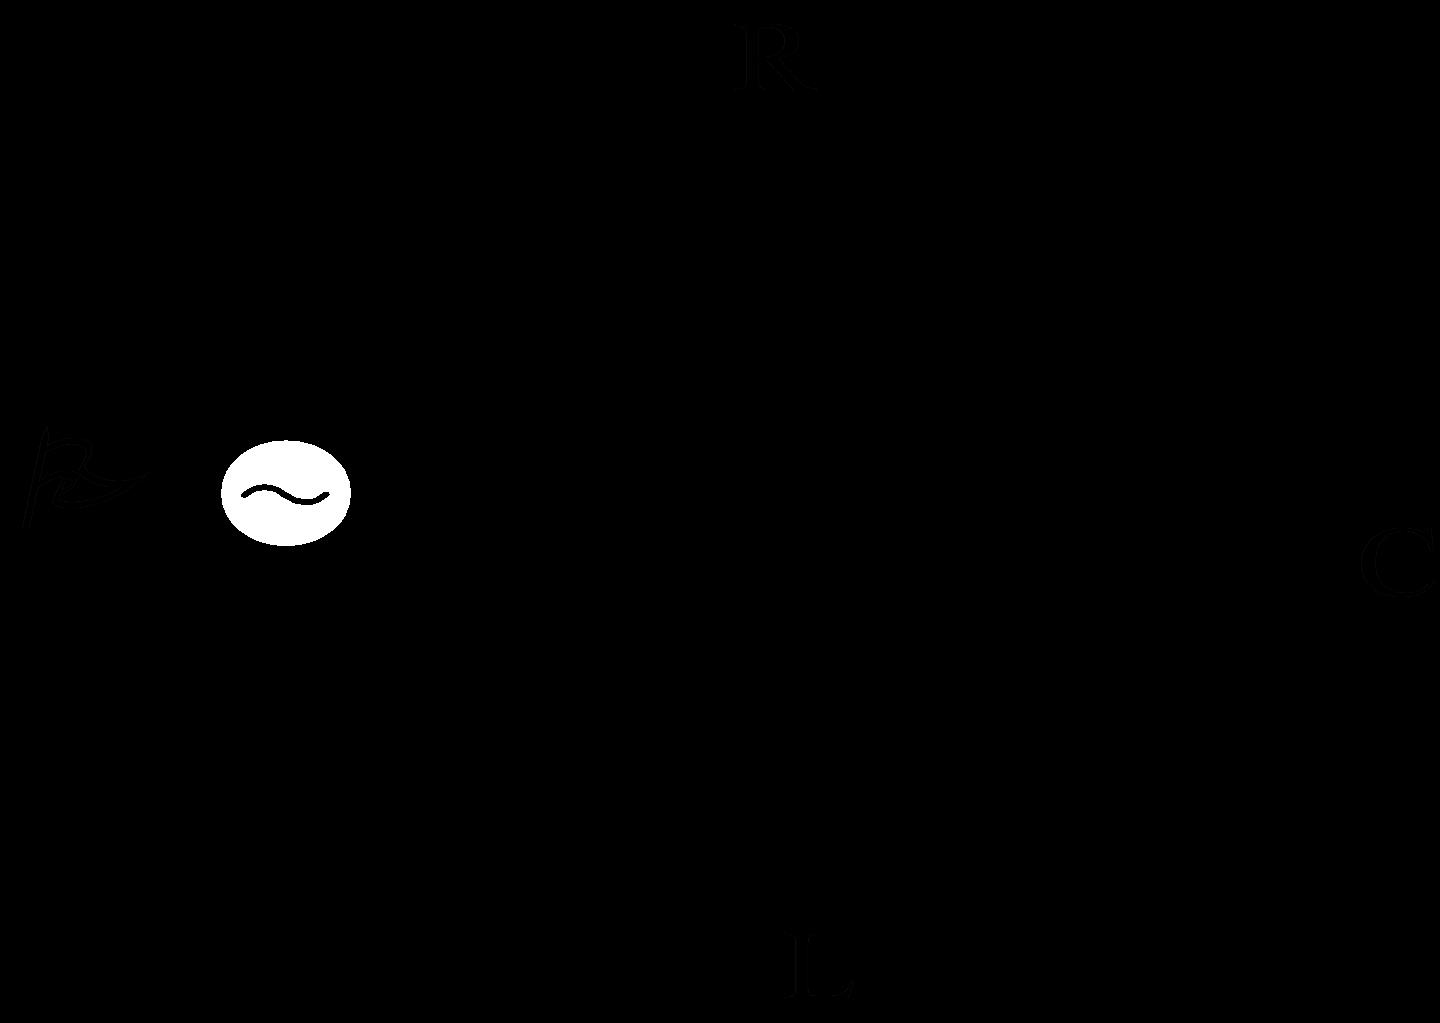
\includegraphics[width=1.8386in,height=1.42in]{PH4CAX4C}
\end{figure}%
where the small coil shaped element is the inductor.

Some of you will remember from PH123 that when a harmonic oscillator was
driven at the natural frequency we had resonance. Let's look at the current
of our $RLC$ circuit. It has an equation very like a harmonic oscillator.
The current is given by%
\begin{equation*}
I_{rms}=\frac{\Delta V_{rms}}{Z}
\end{equation*}%
or 
\begin{equation*}
I_{rms}=\frac{\Delta V_{rms}}{\sqrt{\left( R\right) ^{2}+\left(
X_{L}-X_{C}\right) ^{2}}}
\end{equation*}%
where $X_{L}=2\pi fL$ and $X_{C}=\frac{1}{2\pi fC}.$ When $X_{L}=X_{C}$ this
will be a maximum. This is a form of resonance. You will remember resonance
from swinging as a child. When your parent pushed you at just the right
time, you went higher. We would say your swing \textquotedblleft
amplitude\textquotedblright\ got bigger. The same thing is happening here.
The signal generator is \textquotedblleft pushing\textquotedblright\ the
current through the capacitor. If it pushes at just the right frequency, the
current will get large.

Starting with $X_{L}=X_{C}$, we can find the frequency that will be the
resonant frequency, the frequency of the \textquotedblleft
push\textquotedblright\ that will make the current biggest.%
\begin{eqnarray*}
X_{L} &=&X_{C} \\
2\pi fL &=&\frac{1}{2\pi fC}
\end{eqnarray*}%
then%
\begin{equation*}
f^{2}=\frac{1}{4\pi ^{2}LC}
\end{equation*}%
or%
\begin{equation}
f=\frac{1}{2\pi \sqrt{LC}}  \label{Resonance Frequecy}
\end{equation}

Why do we care? This is a tuning circuit used in radios! We can include a
variable capacitor or a variable inductor in the circuit, and make it
resonate with a desired frequency. Usually a variable capacitor is used. So
when you turn the dial on your radio to adjust the frequency, you are
changing the capacitance of a variable capacitor!

If we had a superconductor with no resistance, the oscillation would go on
forever. Energy would be stored in the capacitor, say, to start out, but as
the current flows a magnetic field is produced. Energy is stored in this
magnetic field. The energy for a resistance-less system would travel from
the electric field to the magnetic field and back.\begin{figure}[h!]
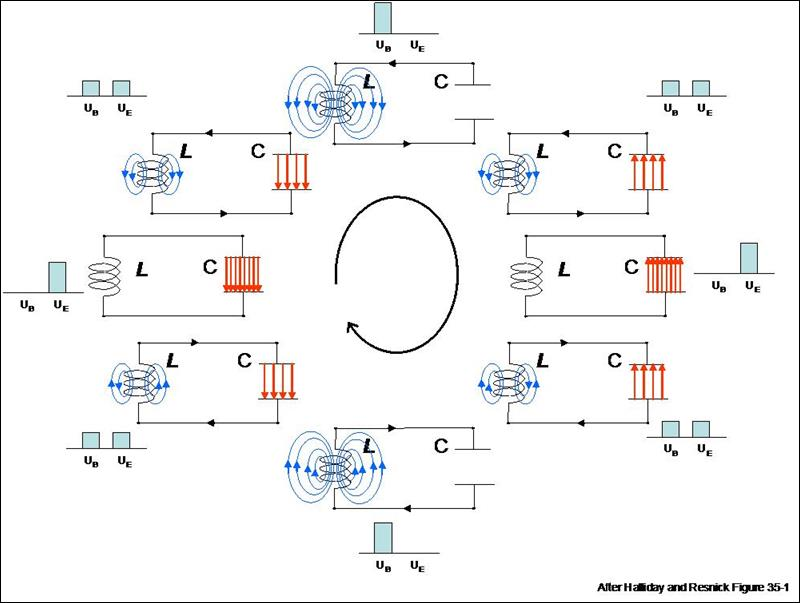
\includegraphics[width=3.2543in,height=%
2.4526in]{PH4CAX4D}
\end{figure}The cycle would go on forever.
But we will need to be careful. We have real resistance in our lab wires,
and the resistance acts like, well, resistance. Resistance is a
non-conservative force, so the resistance will dissipate energy and our
oscillation will eventually die out. But since we are adding in energy from
the signal generator, the effect of resistance will be to make the maximum
voltage of our sine wave less. So in designing your circuit, you will want
to make sure your $R$ is not too big.

I'm going to suggest that we take the resonance part of our inductance model
to perform our model test. Consider the resonant frequency of a LRC circuit.
If we could find the frequency at which our LRC\ circuit goes into
resonance, then we could solve for $L$%
\begin{equation*}
L=\frac{1}{4\pi ^{2}f^{2}C}
\end{equation*}

Since the capacitance is marked on the capacitor, we can calculate $L$
knowing $f.$ We could compare to our calculated value using 
\begin{equation*}
L=\mu _{o}n^{2}V
\end{equation*}%
to see if our solenoid inductance model worked. All we have to do is to
measure $f.$

Really we know enought to make our experiment work. We find $f$ such that
the system is in resonance and then use 
\begin{equation*}
L=\frac{1}{4\pi ^{2}f^{2}C}
\end{equation*}%
to find the inductance of the coil. But we can envison this better if we do
a little bit of higher math and draw another graph. Suppose we hook up our
series LRC\ circuit as described above, and we acknowledge that we do have
resistance. We would find that we could describe our physical situation with
a differential equation. Not everyone is taking differential equations
(M316) concurrently with this class, but most of us will take this class at
some time. We would find that the differential equation for the amount of
charge on the capacitor for our circuit would look like this%
\begin{equation*}
L\frac{d^{2}Q}{dt^{2}}+R\frac{dQ}{dt}+\frac{Q}{C}=\mathcal{E}\sin \left(
\omega ^{\prime }t\right)
\end{equation*}%
where $\mathcal{E}$ is the maximum emf of our signal generator setting and $%
\omega ^{\prime }$ is the frequency setting of our frequency generator. Now
think, resonance means that the amount of charge on the capacitor gets big.
After taking a differential equations class, you will be able to solve for
the charge on the capacitor as a function of frequency. And then, using 
\begin{equation*}
Q=C\Delta V
\end{equation*}%
you will be able to find the voltage across the capacitor as a function of
signal generator driving frequency, $f^{\prime }=\frac{\omega ^{\prime }}{%
2\pi }.$ Your solution will look something like this 
\begin{equation*}
\Delta V_{C}=\frac{\frac{E}{CL}}{\sqrt{\left( \left( 2\pi \left( f\right)
\right) ^{2}-\left( 2\pi f^{\prime }\right) ^{2}\right) ^{2}+2\left( \frac{R%
}{L}\right) \left( 2\pi f^{\prime }\right) ^{2}}}\sin \left( \omega ^{\prime
}t-\phi \right)
\end{equation*}%
Notice the term $\left( \left( 2\pi \left( f\right) \right) ^{2}-\left( 2\pi
f^{\prime }\right) ^{2}\right) ^{2}$ in the denominator. When the resonance
frequency $f$ and the driving frequency $f^{\prime }$ are the same, this
term will be zero, and the denominator will be small. That makes the size of
our $\Delta V_{C}$ sine wave big. That is resonance. Let's plot just the
amplitude term (the part in front of the sine function) so we can see what
it looks like. For a circuit with

\begin{eqnarray*}
\mathcal{E} &=&5\unit{V} \\
L &=&2.3\times 10^{-3}\unit{H} \\
R &=&1\unit{M%
%TCIMACRO{\U{3a9}}%
%BeginExpansion
\Omega%
%EndExpansion
} \\
f_{resonance} &=&18.552\unit{kHz} \\
C &=&32\times 10^{-9}\unit{F}
\end{eqnarray*}%
\begin{equation*}
R>\sqrt{\frac{42.3\times 10^{-3}\unit{H}}{32\times 10^{-9}\unit{F}}}%
=1149.\,\allowbreak 7\unit{%
%TCIMACRO{\U{3a9}}%
%BeginExpansion
\Omega%
%EndExpansion
}
\end{equation*}

we get the following graph

\begin{figure}[h!]
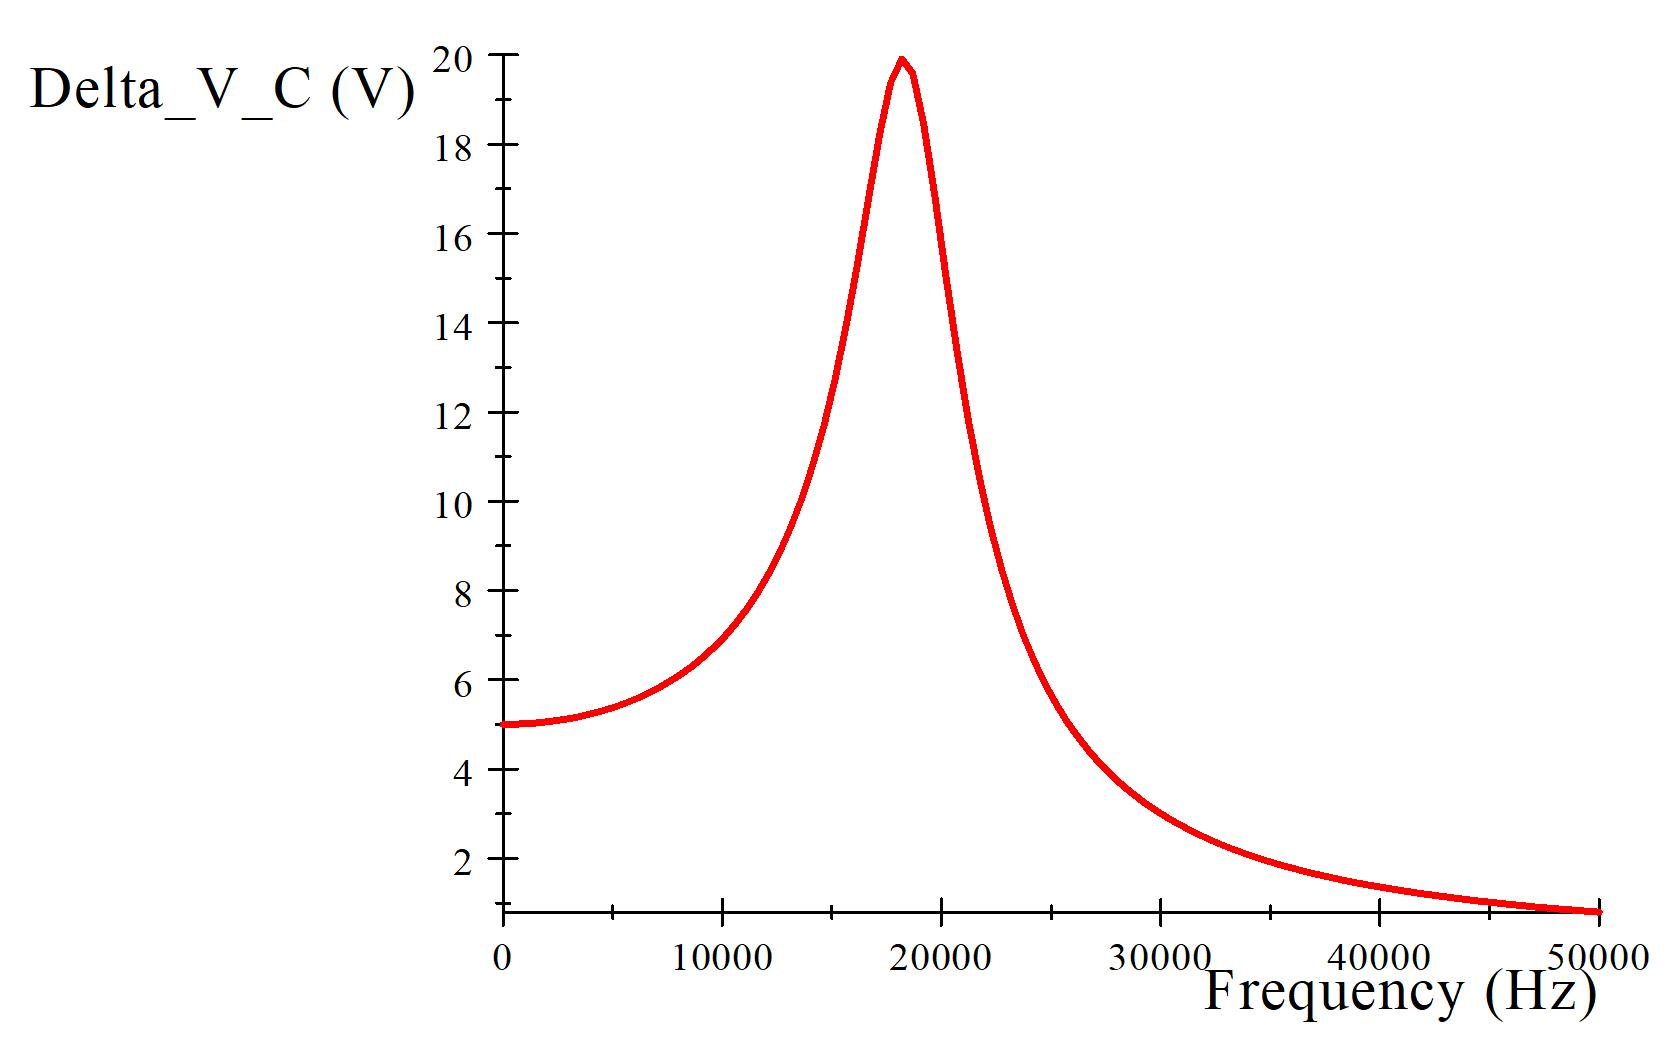
\includegraphics[width=4.4996in,height=3in]{PH4CAX4E}
\end{figure}Let's interpret this graph.
Suppose we start with our signal generator with a low frequency, say, $100%
\unit{Hz},$ We should see a sine wave on the oscilloscope at the same
frequency as the signal generator frequency, but with an amplitude of about $%
5\unit{V}$ (from the midpoint to the peak). Then we change the signal
generator driving frequency until the measured voltage across the capacitor
becomes very large. We want the maximum amplitude. That will be when $%
f=f^{\prime }$ and we can read the resonance frequency off of the indicator
on our signal generator because the signal generator frequency is equal to
the resonance frequency. If we increase the frequency more, the amplitude
will go down, making our sine wave smaller. You should check this to make
sure you have found the maximum amplitude.

\section{Lab Assignment}

\begin{enumerate}
\item Estimate the inductance of your coil using equation \ref{Solenoid
Inductance}.

\item Find The inductance of the coil using an Oscilloscope

\begin{enumerate}
\item Predict the resonant frequency of your $LRC$ circuit using the large
wire coils and something close to a non-electrolitic capacitor. Note that we
are not putting in a resistor, the resistance of the wire in our indictor is
enough to create damping. Also notice that some of the multimeters have a
capacitor tester on them. You might want to check your capacitance for the
capacitor you choose.

\item Set up an $LRC$ circuit . Make sure your resistance is not too high
using equation \ref{Criticall Damping Criteria}. Use one of our signal
generators to produce as the source of variable emf. \begin{figure}[h!]
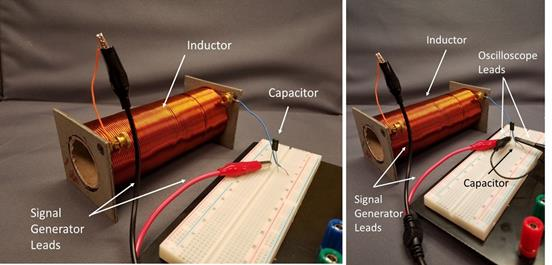
\includegraphics[width=4.6496in,height=%
2.2423in]{PH4CAX4F}
\end{figure}

\item Test the circuit using the oscilloscope. Make sure you see a nice sine
wave. Either side of the capacitor is a nice place to hook the oscilloscope
probe, if your oscilloscope has a ground lead, hook it to the other side of
the capacitor.\begin{figure}[h!]
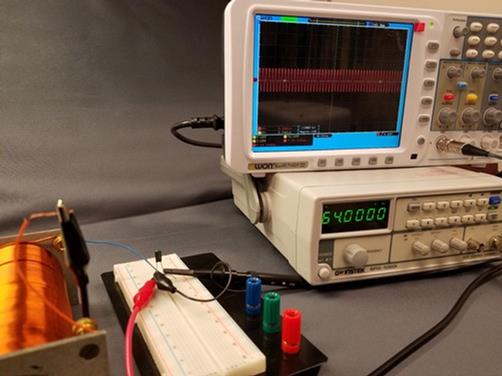
\includegraphics[width=4.23in,height=3.1727in]{PH4CAX4G}
\end{figure}

\item Adjust your signal generator near your natural frequency of
oscillation. Note what happens to the amplitude as you tune the dial.

\item Determine your actual resonant frequency, $f_{A}$.

\item Calculate your inductance based on $f_{A}$. Compare to your calculated
value. If there is a difference, try to explain it.
\end{enumerate}
\end{enumerate}

%TCIMACRO{\TeXButton{vfill}{\vfill}}%
%BeginExpansion
\vfill%
%EndExpansion